\section{results and scalability of Coordinate Descent}


MeerKAT simulation with meqtrees. Simulation suite. Not a lot of noise, fairly simple data to test the algorithm.

Two simulations, one of point sources and one of mixed sources. 

Super resolution. The reconstruction should be able to locate the point sources below the accuracy of the instrument.

\subsubsection{Two Point Sources}


\begin{figure}[h]
	\centering
	\begin{subfigure}[b]{0.45\linewidth}
		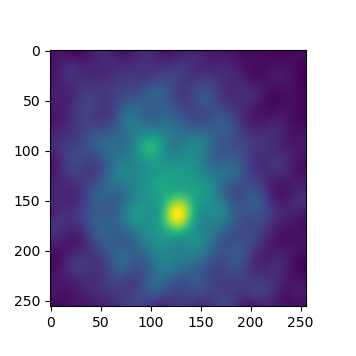
\includegraphics[width=\linewidth]{./chapters/05.algorithms/sim02/sim02_point_dirty.png}
		\caption{Dirty Image of two point sources}
		\label{results:point:dirty}
	\end{subfigure}
	\begin{subfigure}[b]{0.45\linewidth}
		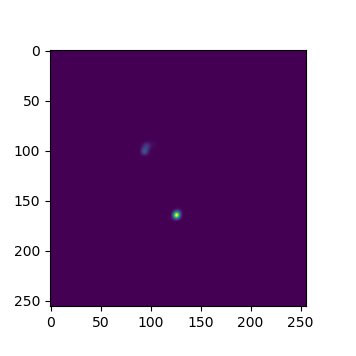
\includegraphics[width=\linewidth]{./chapters/05.algorithms/sim02/image4.png}
		\caption{Reconstruction after 4 Full iterations}
		\label{results:point:cd}
	\end{subfigure}
	\caption{Image reconstruction on two point sources.}
	\label{results:point}
\end{figure}

faint source is spread more widely. Not good, The paper \cite{starck2015starlet} used different $\lambda$ values for different starlet levels. Maybe with this it can be forced to do more precise results, but it was not tried in this work.

\subsubsection{Gaussian and Point Sources}
Mixture of gaussian and point sources. 

\begin{figure}[h]
	\centering
	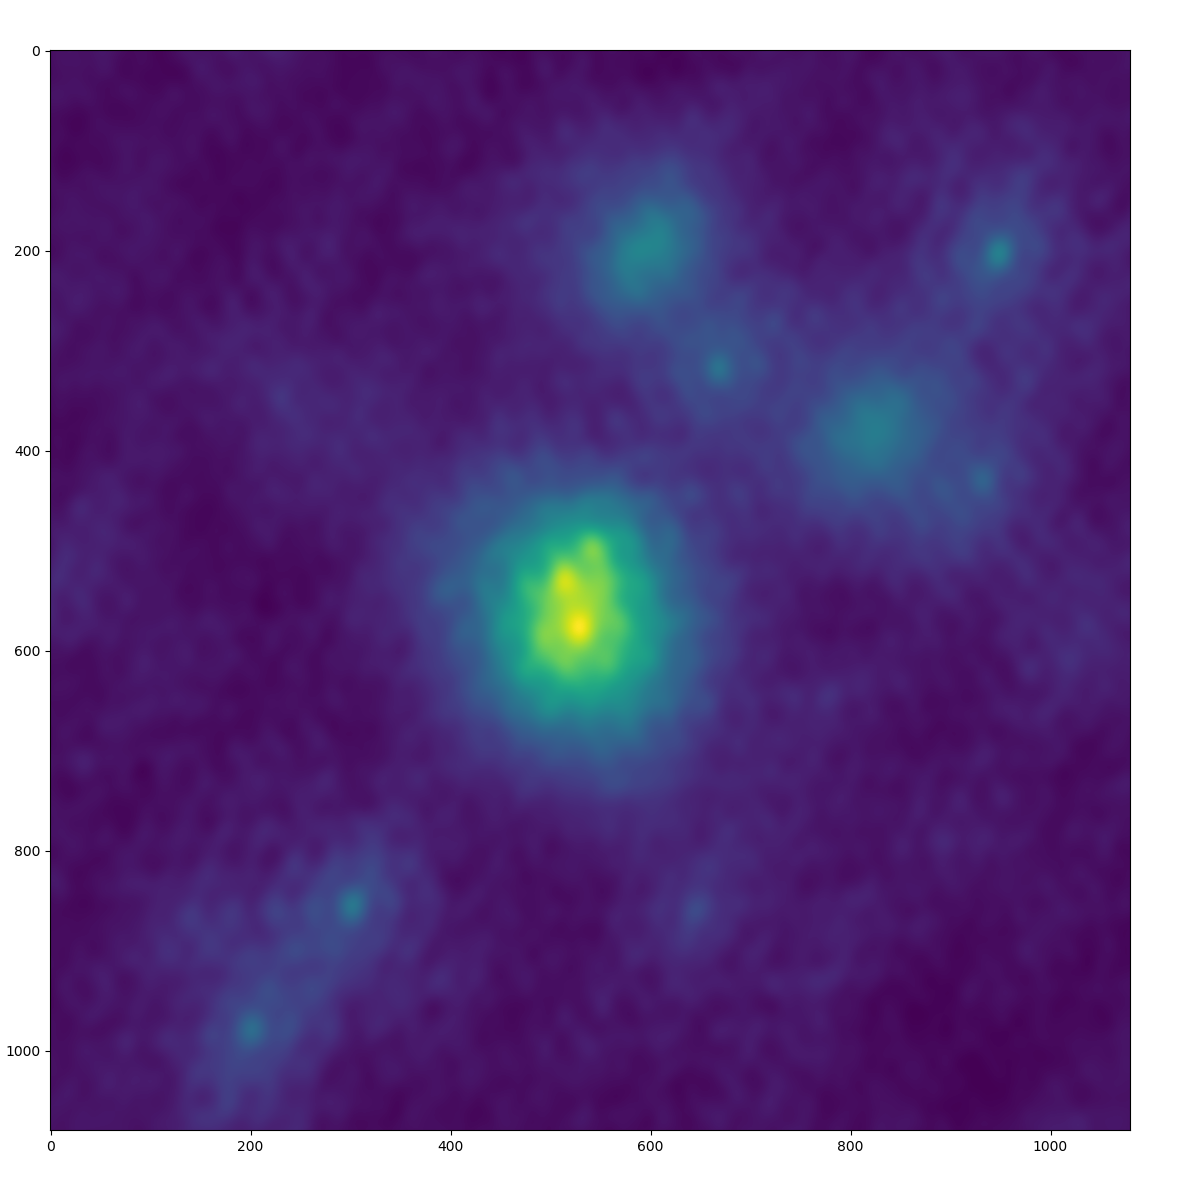
\includegraphics[width=0.5\linewidth]{./chapters/05.algorithms/results/sim00_mixed_sources_dirty.png}
	\caption{Dirty Image}
	\label{alg:gauss:dirty}
\end{figure}

\begin{figure}[h]
	\centering
	\begin{subfigure}[b]{0.45\linewidth}
		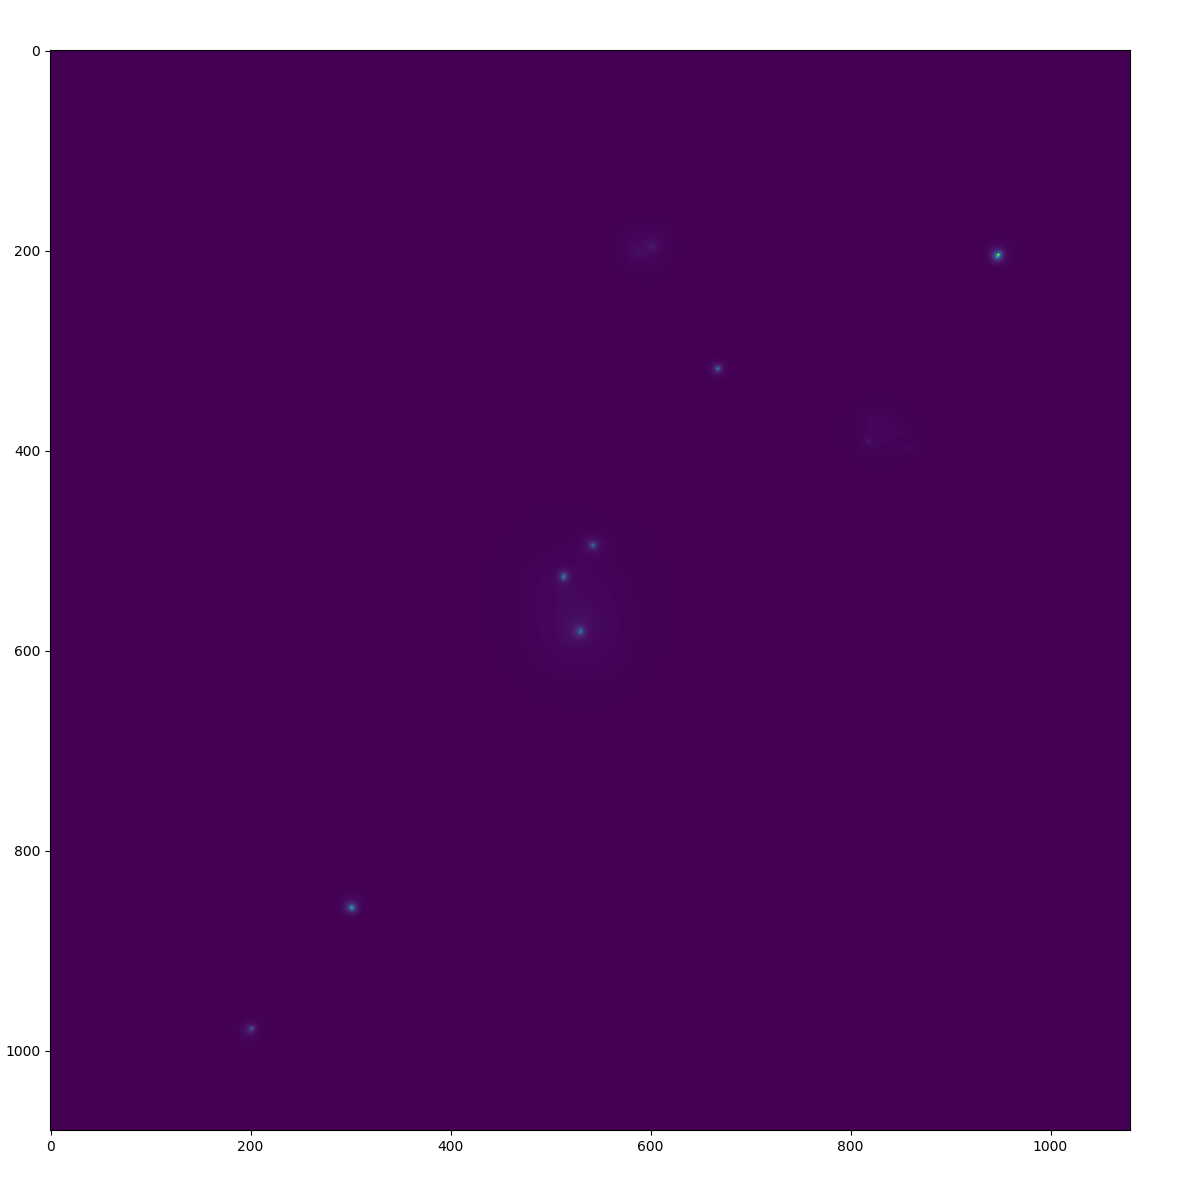
\includegraphics[width=\linewidth]{./chapters/05.algorithms/results/image.png}
		\caption{Reconstruction after one full iteration}
		\label{results:g55:nrao:rec}
	\end{subfigure}
	\begin{subfigure}[b]{0.45\linewidth}
		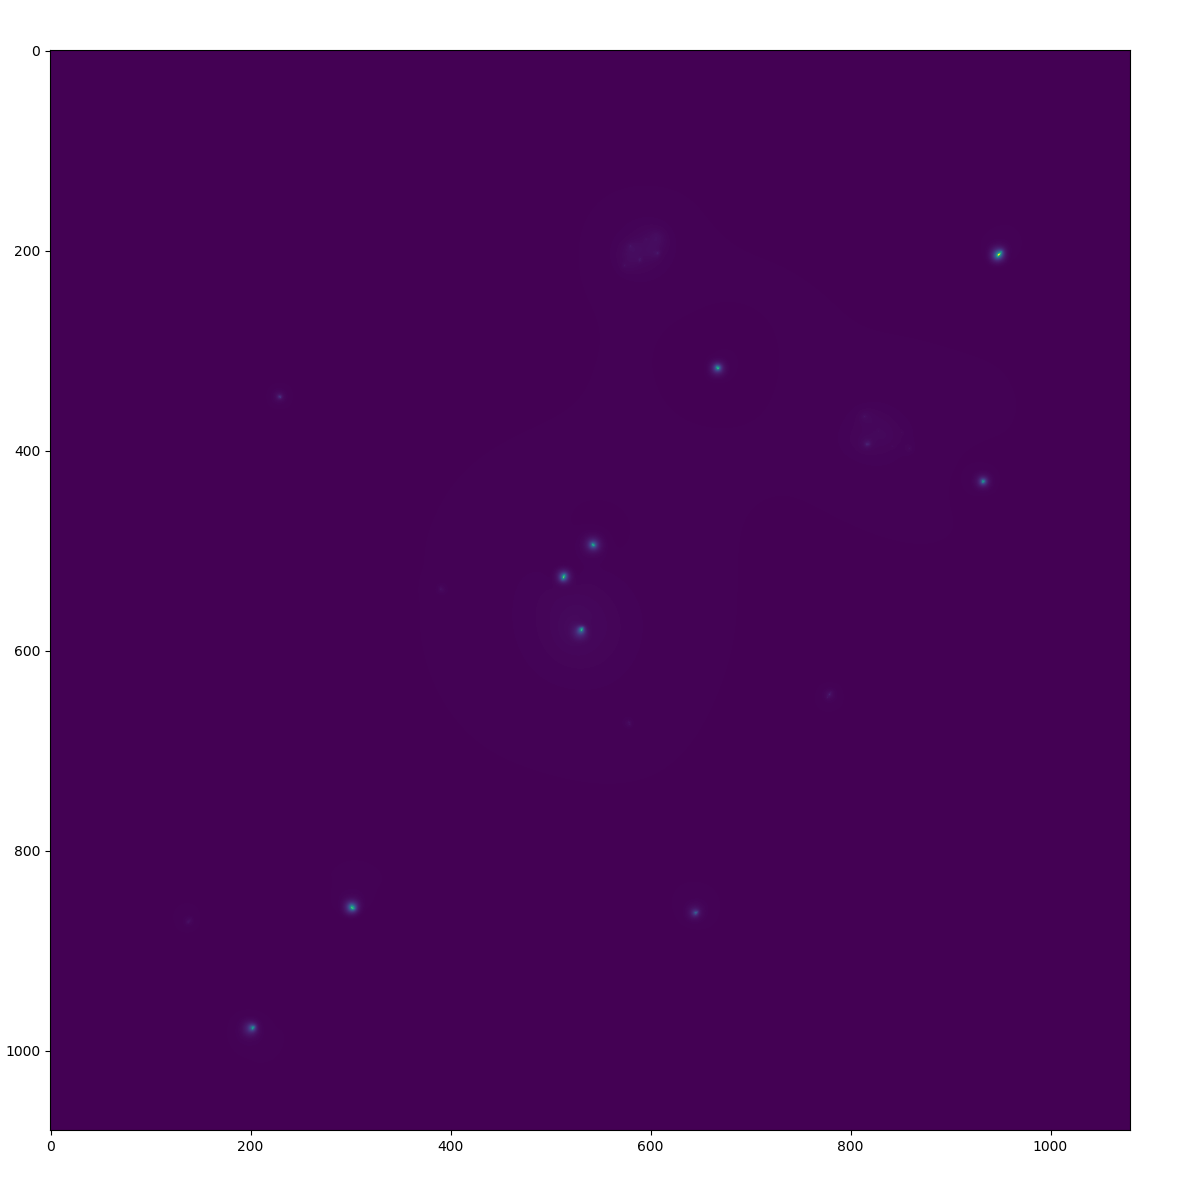
\includegraphics[width=\linewidth]{./chapters/05.algorithms/results/image4.png}
		\caption{Reconstruction after 4 Full iterations}
		\label{results:g55:nrao:dirty}
	\end{subfigure}
	\caption{}
	\label{results:g55:nrao}
\end{figure}

\subsection{Scalability estimates with ideal heuristics}
Bunch of heuristics. There are a lot of little ways to optimize this algorithm. The question is, is it worth going further and try to improve the algorithm further. So we want to estimate the lower bound of the algorithm.

Convergence is hard to determine in general. Following simplified assumptions were made: We have a heuristic with oracle performance. It returns only the locations of $\alpha$ in constant time. Furthermore, we assume all axes are independent from each other, only one descent per non-zero axis is necessary.

$S$


$res * starlet = M$
descent:
$gen fcol = 3*M$
$a = 3 * M$
$b = 4 * M$
$residuals, fcol*diff =  M$

$total_mit_gencol = 11M$

total CD = $S * 11M + 2M * starlets$

$S$ depends on the image content directly. For example if the image contains 15 point sources and five Gaussian extended emissions, then $S$ equals 20 non-zero components (if we assume the Gaussian sources require only one starlet for representation). Coordinate Descent therefore is independent of the image size $N$. It solely depends on the size of the measurements $M$, and the number of non-zero components in the dictionary $S$. 

It does not use any approximation for the fourier transform.



(Cite New W-stacking approach)
Nufft: $M + 2N log 2N$
W-stacking = $M + W*(2N log 2N + 2N) + N log N$
Deconvolution = ??

The major cycle algorithm depends on more parameters. Assumptions were made in favor of Coordinate Descent.

the number of w-stacks $W$. If this is the case

\cite{pratley2018fast} fast w-stacking w-projection

